\documentclass[onecolumn, draftclsnofoot,10pt, compsoc]{IEEEtran}
\usepackage{graphicx}
\usepackage{float}
\usepackage{url}
\usepackage{setspace}
\usepackage[english]{babel}

\usepackage{geometry}
\geometry{textheight=9.5in, textwidth=7in}

% 1. Fill in these details
\def \CapstoneTeamName{		AsyncSync}
\def \CapstoneTeamNumber{		51}
\def \GroupMemberOne{			Christopher Pavlovich}
\def \GroupMemberTwo{			Eli Sandine}
\def \GroupMemberThree{			Jaehyung You}
\def \GroupMemberFour{			Yeongae Lee}
\def \CapstoneProjectName{		Project BoxSand: Shared Whiteboard}
\def \CapstoneSponsorCompany{	OSU: Physics Department}
\def \CapstoneSponsorPerson{		Kenneth Walsh}

% 2. Uncomment the appropriate line below so that the document type works
\def \DocType{	%Problem Statement
				%Requirements Document
				%Technology Review
				Design Document
				%Progress Report
				}

\newcommand{\NameSigPair}[1]{\par
\makebox[2.75in][r]{#1} \hfil 	\makebox[3.25in]{\makebox[2.25in]{\hrulefill} \hfill		\makebox[.75in]{\hrulefill}}
\par\vspace{-12pt} \textit{\tiny\noindent
\makebox[2.75in]{} \hfil		\makebox[3.25in]{\makebox[2.25in][r]{Signature} \hfill	\makebox[.75in][r]{Date}}}}
% 3. If the document is not to be signed, uncomment the RENEWcommand below
%\renewcommand{\NameSigPair}[1]{#1}

%%%%%%%%%%%%%%%%%%%%%%%%%%%%%%%%%%%%%%%
\begin{document}
\begin{titlepage}
    \pagenumbering{gobble}
    \begin{singlespace}
        \hfill
        % 4. If you have a logo, use this includegraphics command to put it on the coversheet.
        %\includegraphics[height=4cm]{CompanyLogo}
        \par\vspace{.2in}
        \centering
        \scshape{
            \huge CS Capstone \DocType \par
            {\large\today}\par
            \vspace{.5in}
            \textbf{\Huge\CapstoneProjectName}\par
            \vfill
            {\large Prepared for}\par
            \Huge \CapstoneSponsorCompany\par
            \vspace{5pt}
            {\Large\NameSigPair{\CapstoneSponsorPerson}\par}
            {\large Prepared by }\par
            Group\CapstoneTeamNumber\par
            % 5. comment out the line below this one if you do not wish to name your team
            \CapstoneTeamName\par
            \vspace{5pt}
            {\Large
              \NameSigPair{\GroupMemberOne}\par
              \NameSigPair{\GroupMemberTwo}\par
              \NameSigPair{\GroupMemberThree}\par
			  \NameSigPair{\GroupMemberFour}\par
            }
            \vspace{20pt}
        }
        \begin{abstract}
		The following document describes the design and structure of the AsyncSync software, the purpose and scope of the document and the intended audience. Furthermore, the document uses diagrams to detail interaction between the users and the software, as well as the AsyncSync software interacting with the Canvas Learning Management Software.
    \end{abstract}
    \end{singlespace}
\end{titlepage}
\newpage
\pagenumbering{arabic}
%\tableofcontents
% 7. uncomment this (if applicable). Consider adding a page break.
%\listoffigures
%\listoftables
%\clearpage

\section{Overview}

	AsyncSync is a web based application that is real-time collaborative software in the form of an interactive whiteboard. The application will allow multiple users to share an online whiteboard on which they will be able to draw shapes, and objects, write equations, share ideas and communicate. AsyncSync will permit users to simultaneously edit a single workspace (similar to Google Docs), record everything drawn or written on the whiteboard and allow the users to communicate. AsyncSync is intended to replace the current online homework system used by introductory physics students at Oregon State University (OSU). The application will be interacting with the Canvas Learning Management Software (LMS) that is used at OSU. Furthermore, the primary goal of the AsyncSync software is generating data about the user interaction with the software, to aid researchers studying the efficacy of the software, and homework system.

\subsection{Purpose}

	The purpose of this document is to provide a description of the design and structure of the AsyncSync software and how users will interact with the system. Additionally, it details the interaction between the AsyncSync software and Canvas LMS. Diagrams are provided to better illustrate these interactions. Furthermore, this document will be used by the development team as a framework to begin implementing the software and track their progress throughout the development cycle.

	\subsection{Scope}

	The scope of this document includes the structure and design of the AsyncSync software and covers the user interactions with the software. Furthermore, the document details how the AsyncSync software will interact with the Canvas LMS, and is illustrated with diagrams. Also within the scope, the use of tracking user’s interactions with the software and how data will be gathered to for researchers is discussed. This document does not cover in-depth detail of the technologies being used to implement the software.

	\subsection{Audience}

	Primarily, this document is intended for the AsyncSync development team that will be creating the software and the stakeholder, Kenneth Walsh. Additionally, the document is meant for future developers that will continue building upon this software in the years to come to help them understand the original design and implementation of the software.


\section{Definitions}

	\begin{enumerate}
		\item AWW: A Web Whiteboard, the whiteboard API
		\item BoxSand: A website created by the Physics department at Oregon State University to replace textbooks with free learning material.
	\end{enumerate}

\section{UML and ERD Diagram}
	\subsection{UML Diagram}

		\begin{figure}[H]
			\begin{center}
				\caption{UML Diagram}
				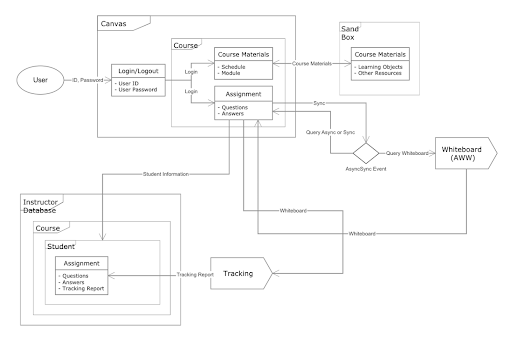
\includegraphics[width=6in]{UML Diagram.png}
			\end{center}
		\end{figure}

		\begin{enumerate}
			\item
			User: Students
			\item
			Canvas: Users can access courses after login into Canvas. They can get course materials, take quizzes and do assignments.
			\item
			BoxSand: A website created by the Physics department at Oregon State University to replace textbooks with free learning material.
			\item
			AsyncSync event: This event asks users to change mode. When they login to Canvas, their mode automatically set up to Async mode. When more than one student works on the same question, it suggests students switch from Async mode to Sync mode.
			\item
			Instructor database: Tracking report is saved into this database. Only instructors can access it, so they can track students’ whiteboard.
			\item
			Whiteboard (AWW): It provides a shared whiteboard to students in Sync mode.
			\item
			Tracking: It converts whiteboard information into tracking reports and then sends it to the instructor database.
		\end{enumerate}

	\subsection{ERD Diagram}

		\begin{figure}[H]
			\begin{center}
				\caption{ERD Diagram}
				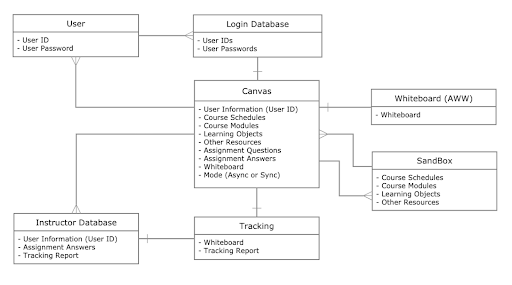
\includegraphics[width=6in]{ERD Diagram.png}
			\end{center}
		\end{figure}

		\begin{enumerate}
			\item
			User: A user types user ID and password.
			\item
			Login Database: If user ID and password match, send user ID to the Canvas website, so a user can access to courses.
			\item
			Canvas: Canvas is the hub of the data exchange.
			\item
			Whiteboard (AWW): It provides whiteboards to Canvas.
			\item
			BoxSand: BoxSand send and receive course materials from Canvas
			\item
			Instructor database: It gets user information and tracking reports form Canvas and tracking software. It matches both information and saves.
			\item
			Tracking: It receives whiteboard and then converts to tracking reports.
		\end{enumerate}


\section{Concerns/constraints}

	Our primary concern is in the ability to gather enough tracking data. The majority of our work will be in connecting students in a shared learning space. The ability to track these interactions relies heavily on seeing which students click what and which tools they use most frequently. This requires all students to remain anonymous in their interactions, which could complicate some of the data gathering. Beyond anonymity, we are restricted to counting API calls in regard to user tracking. Canvas is a proprietary service for security purposes, meaning we cannot see the majority of what happens in the background. However, we are able to run a local Docker instance of Canvas which should make testing much easier.

	Due to the security requirements in place by the University, we will not be able to host our web application outside of the Canvas environment. This prevents the open-source and more widely available product we hoped for, but is not a foreseeable issue regarding functionality for the university.

	Among other security interests is the need to protect gathered tracking data. With this, there will be no mass database that we have access to for tracking data storage. Instead, the script will output data into a machine readable format to be handled by E-Campus or a future project. This will accommodate for the extensive security analysis required by FERPA regulations.


\section{Whiteboard interface and functionality}

	Whiteboard is a tool offered in Sync mode. It is provided when the user accepts the Sync mode query. Canvas should be able to check the number of students working on the same problem. Then, if more than one student works on the same problem, it has to suggest Sync mode to students. If students reject Sync mode, Canvas cannot suggest it anymore. However, students can change from Async mode to Sync mode by clicking on the change mode button. If students accept Sync mode, Canvas requests a whiteboard to AWW. Then, it is offered to students.

	\begin{figure}[H]
		\begin{center}
			\caption{Sequence Diagram: Load a Whiteboard}
			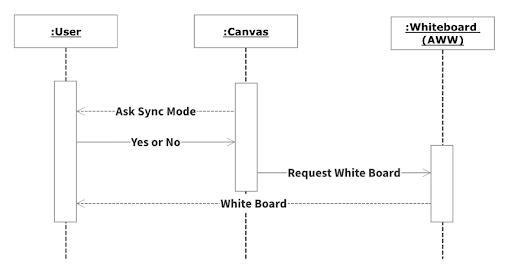
\includegraphics[width=6in]{Sequence Diagram1.png}
		\end{center}
	\end{figure}

	\begin{figure}[H]
		\begin{center}
		\caption{AWW Whiteboard}
			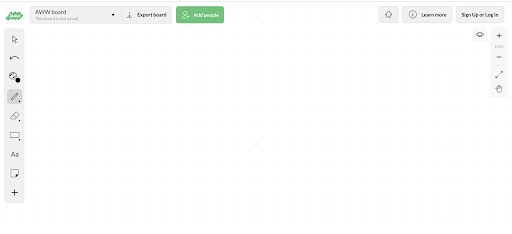
\includegraphics[width=6in]{AWW Whiteboard.png}
		\end{center}
	\end{figure}

	After a whiteboard finish loading into the Canvas website, students are free to draw on it. Canvas read every single change and send it to tracking software.

	\begin{figure}[H]
		\begin{center}
			\caption{Sequence Diagram: Read Changed on a Whiteboard}
			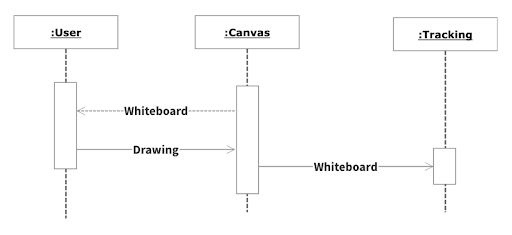
\includegraphics[width=6in]{Sequence Diagram2.png}
		\end{center}
	\end{figure}

\section{Tracking System}

	The administrator, such as professor or other authorized personnel, is the only one to allowed access into the tracking database. In other words, students are never allowed to get into the database. Once student is working on our whiteboard system (AWW), the tracking system will automatically record their work into the database. Since students draw their work on AWW, the database will connect to AWW directly. Students can never control this tracking system. Only the administrator can control the tracking system. For the structure of the database, all tracking data will be mapped to the corresponding students to avoid the conflict. For the professor, he/she can access to the database and see the tracking data by searching student’s name. Tracking system doesn’t need a immediate response. Since the drawing involves many processes, it is very inefficient for the system to save it as data every time students draw. Therefore, the system will be designed in such a way that the data will be stored every some cycle or the drawing task is completed. After the data is fully accessible and visible by the professor, he/she can give students a feedback.

	\begin{figure}[H]
		\begin{center}
			\caption{Sequence Diagram: Tracking system in the detailed view}
			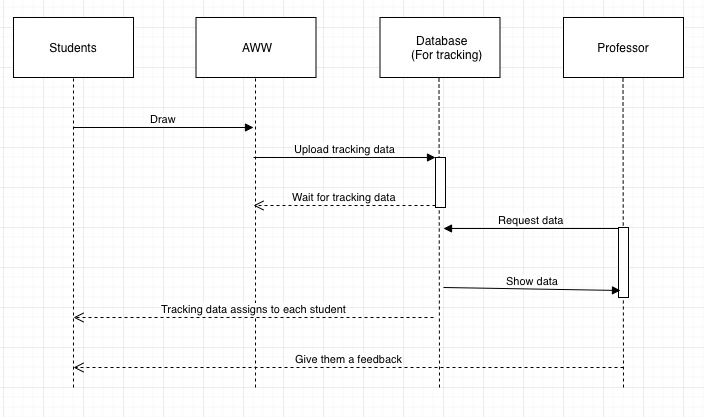
\includegraphics[width=5in]{tracking.jpg}
		\end{center}
	\end{figure}

\section{Database}

	The database is going to be an integral part of the software because collecting data is the main goal of the project and it will need to be stored for later retrieval. Once the data is generated from the tracking the users on the frontend, it will be moved to the backend to be stored in a database. A MySQL database will be implemented to store all the information that is being tracked on the frontend of the application. The data will be stored into the relevant tables that the client will be able to access the data and perform queries to retrieve any relevant data for research purposes. Additionally, users will be able to rewind, or replay the drawings they have previously created and saved to the database.

\section{Conclusion}

	In conclusion, the AsyncSync project is a web software which allows students to collaborate in real-time. It lets students communicate online by offering a whiteboard. Every single change on the whiteboard is saved into the database. AsyncSync project divides into three design parts which are whiteboard and tracking. A whiteboard should be loaded from AWW in whiteboard design. Canvas suggests Sync mode. If students accept, AWW loads a whiteboard into Canvas. Tracking design reports all changes on a whiteboard. Reported changes are saved into the instructor database. AsyncSync is the new style of the education program. It will replace the online physics assignment system. AsyncSync project is expected to improve student learning efficiency.

\section{Gantt Charts}

	\begin{figure}[H]
		\begin{center}
			\caption{Gantt Chart - Term 1}
			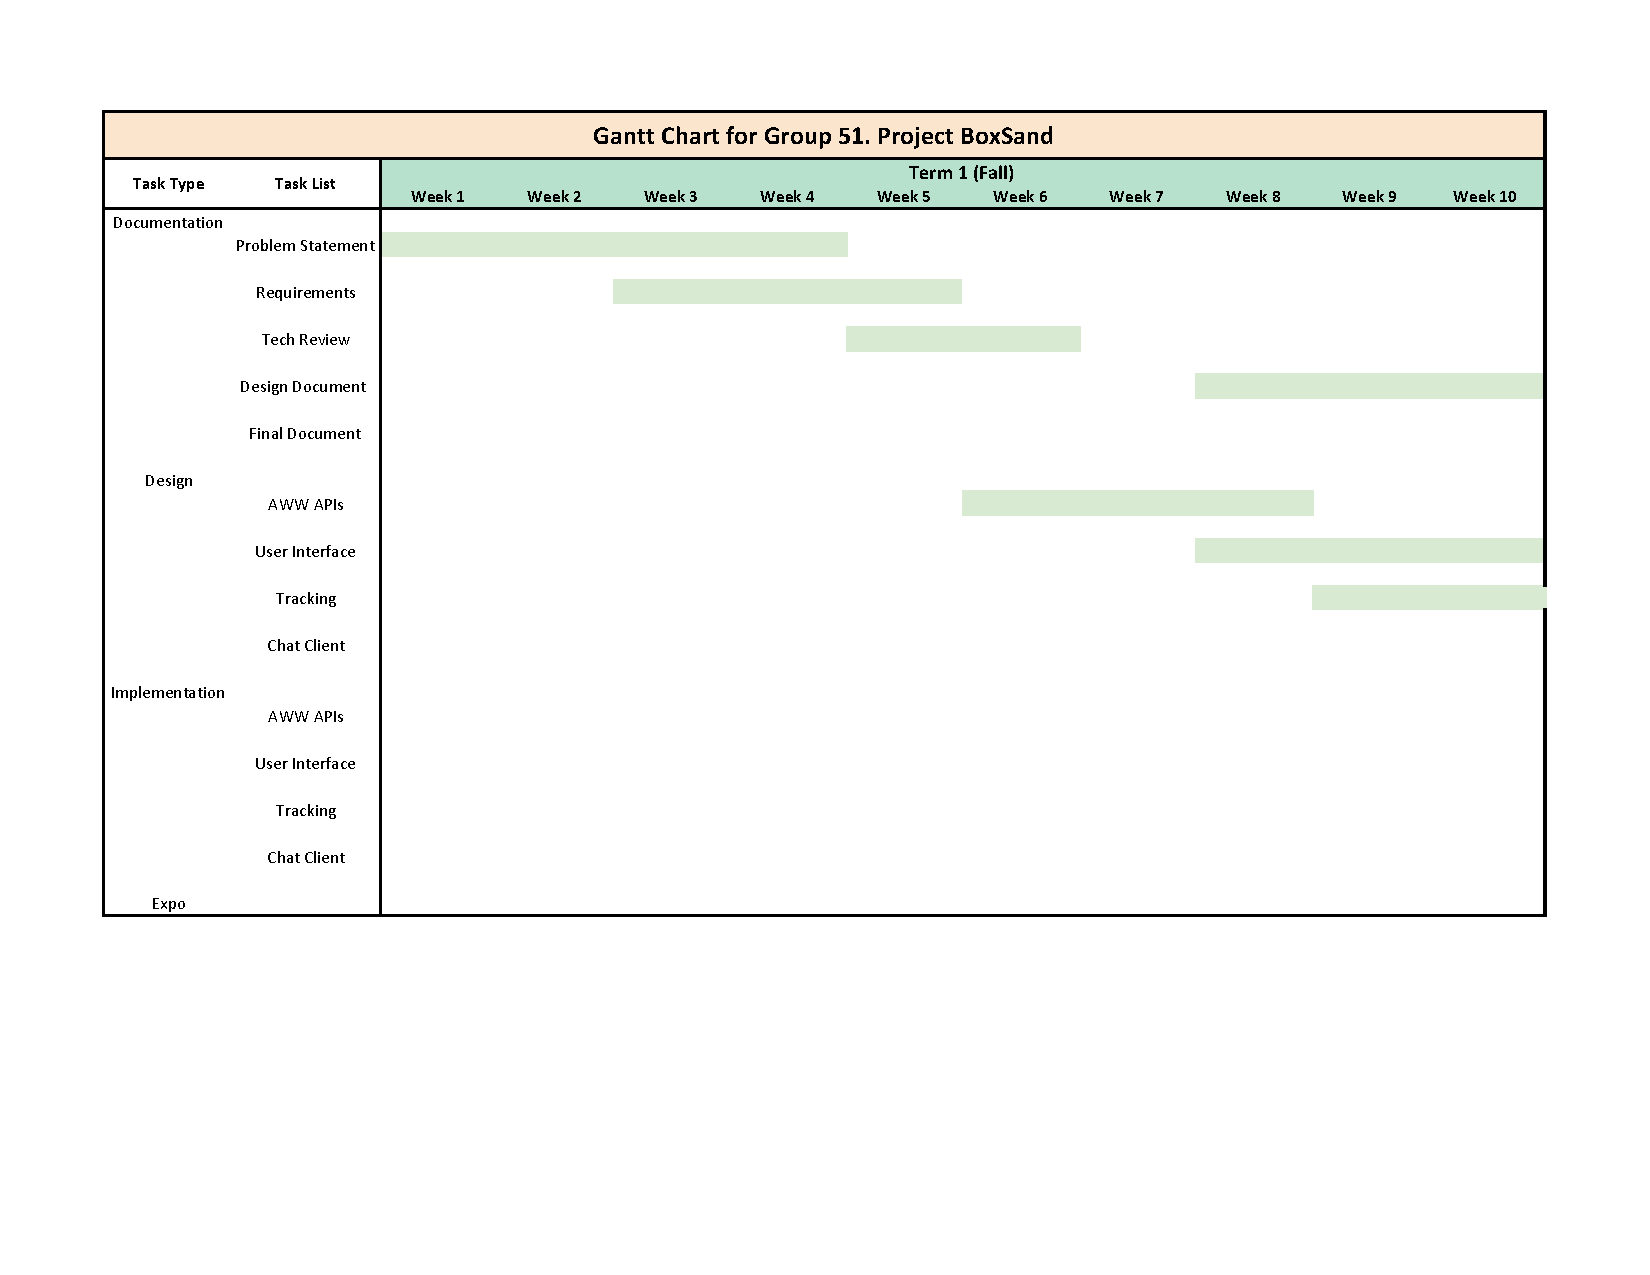
\includegraphics[width=7in]{Simplified Gantt Chart - Term 1.pdf}
		\end{center}
	\end{figure}


	\begin{figure}[H]
		\begin{center}
			\caption{Gantt Chart - Term 2}
			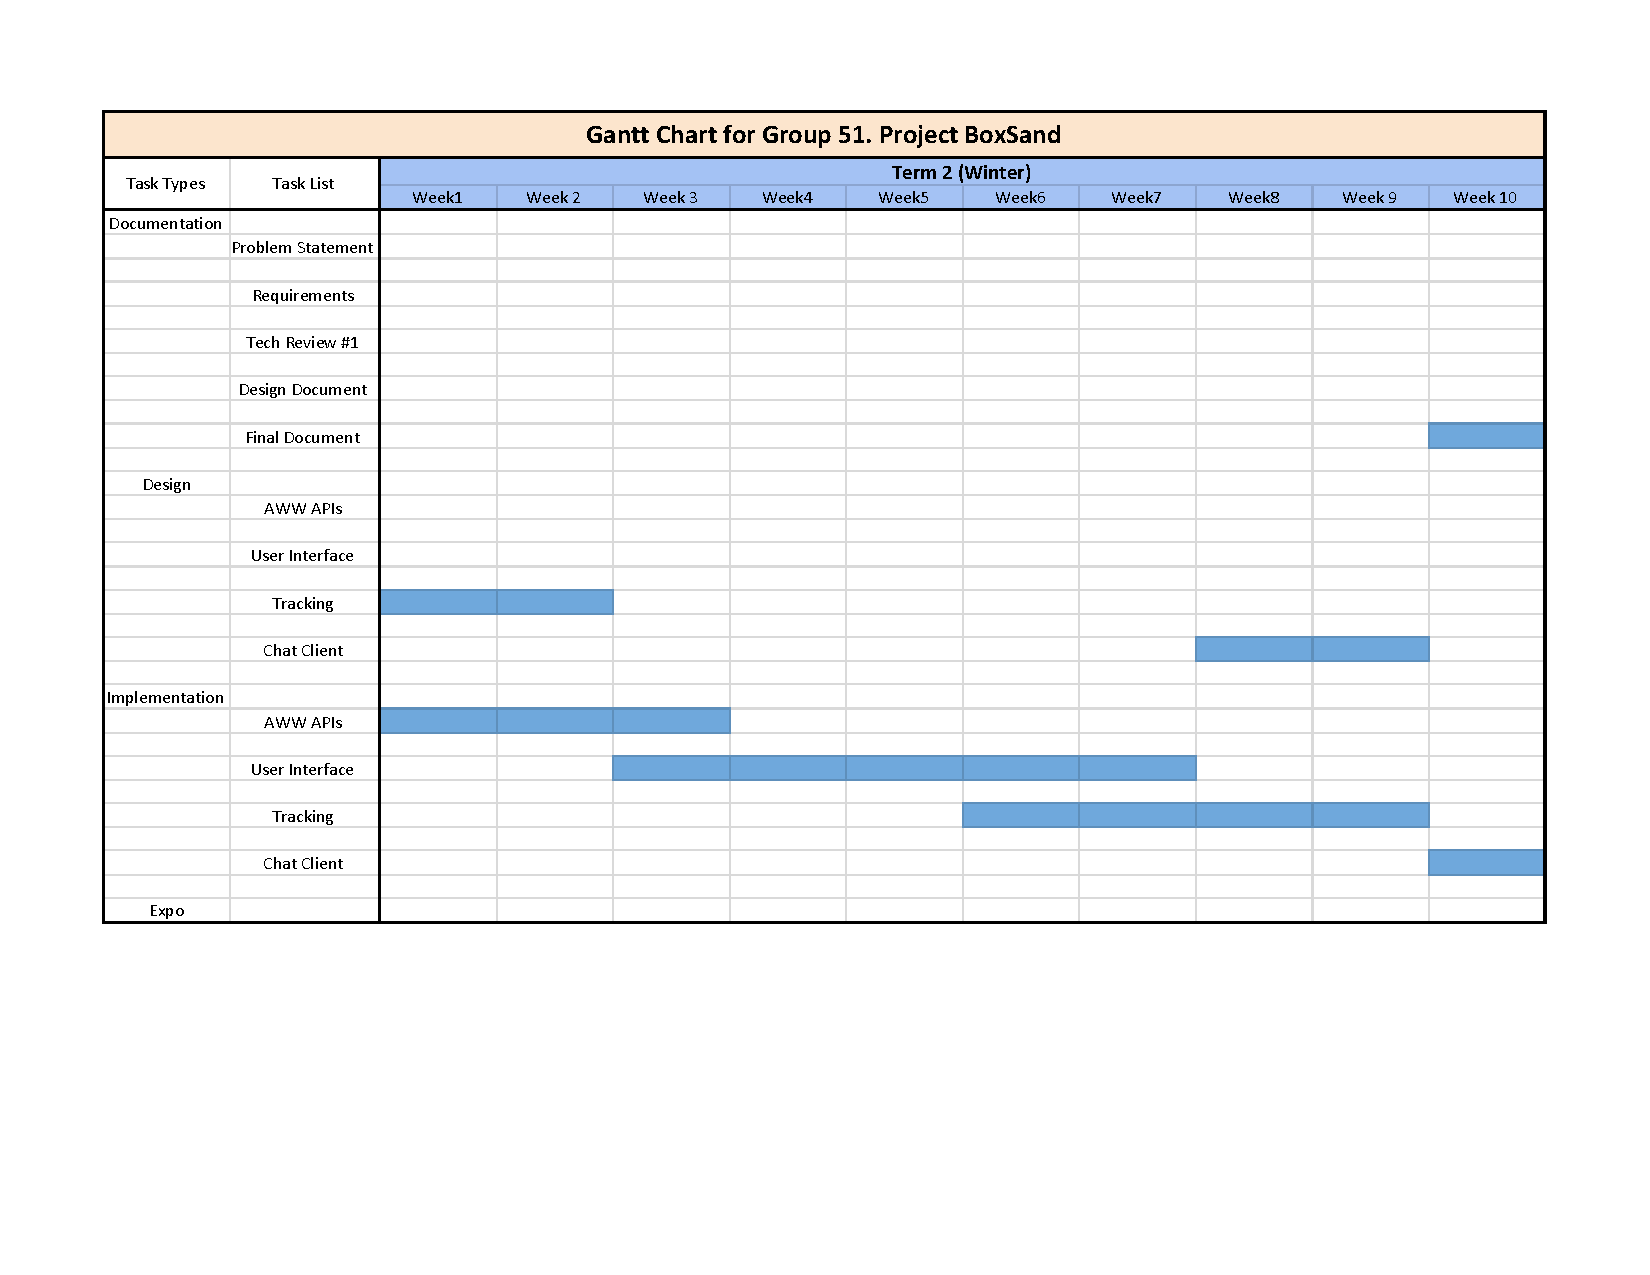
\includegraphics[width=7in]{Simplified Gantt Chart - Term 2.pdf}
		\end{center}
	\end{figure}


	\begin{figure}[H]
		\begin{center}
			\caption{Gantt Chart - Term 3}
			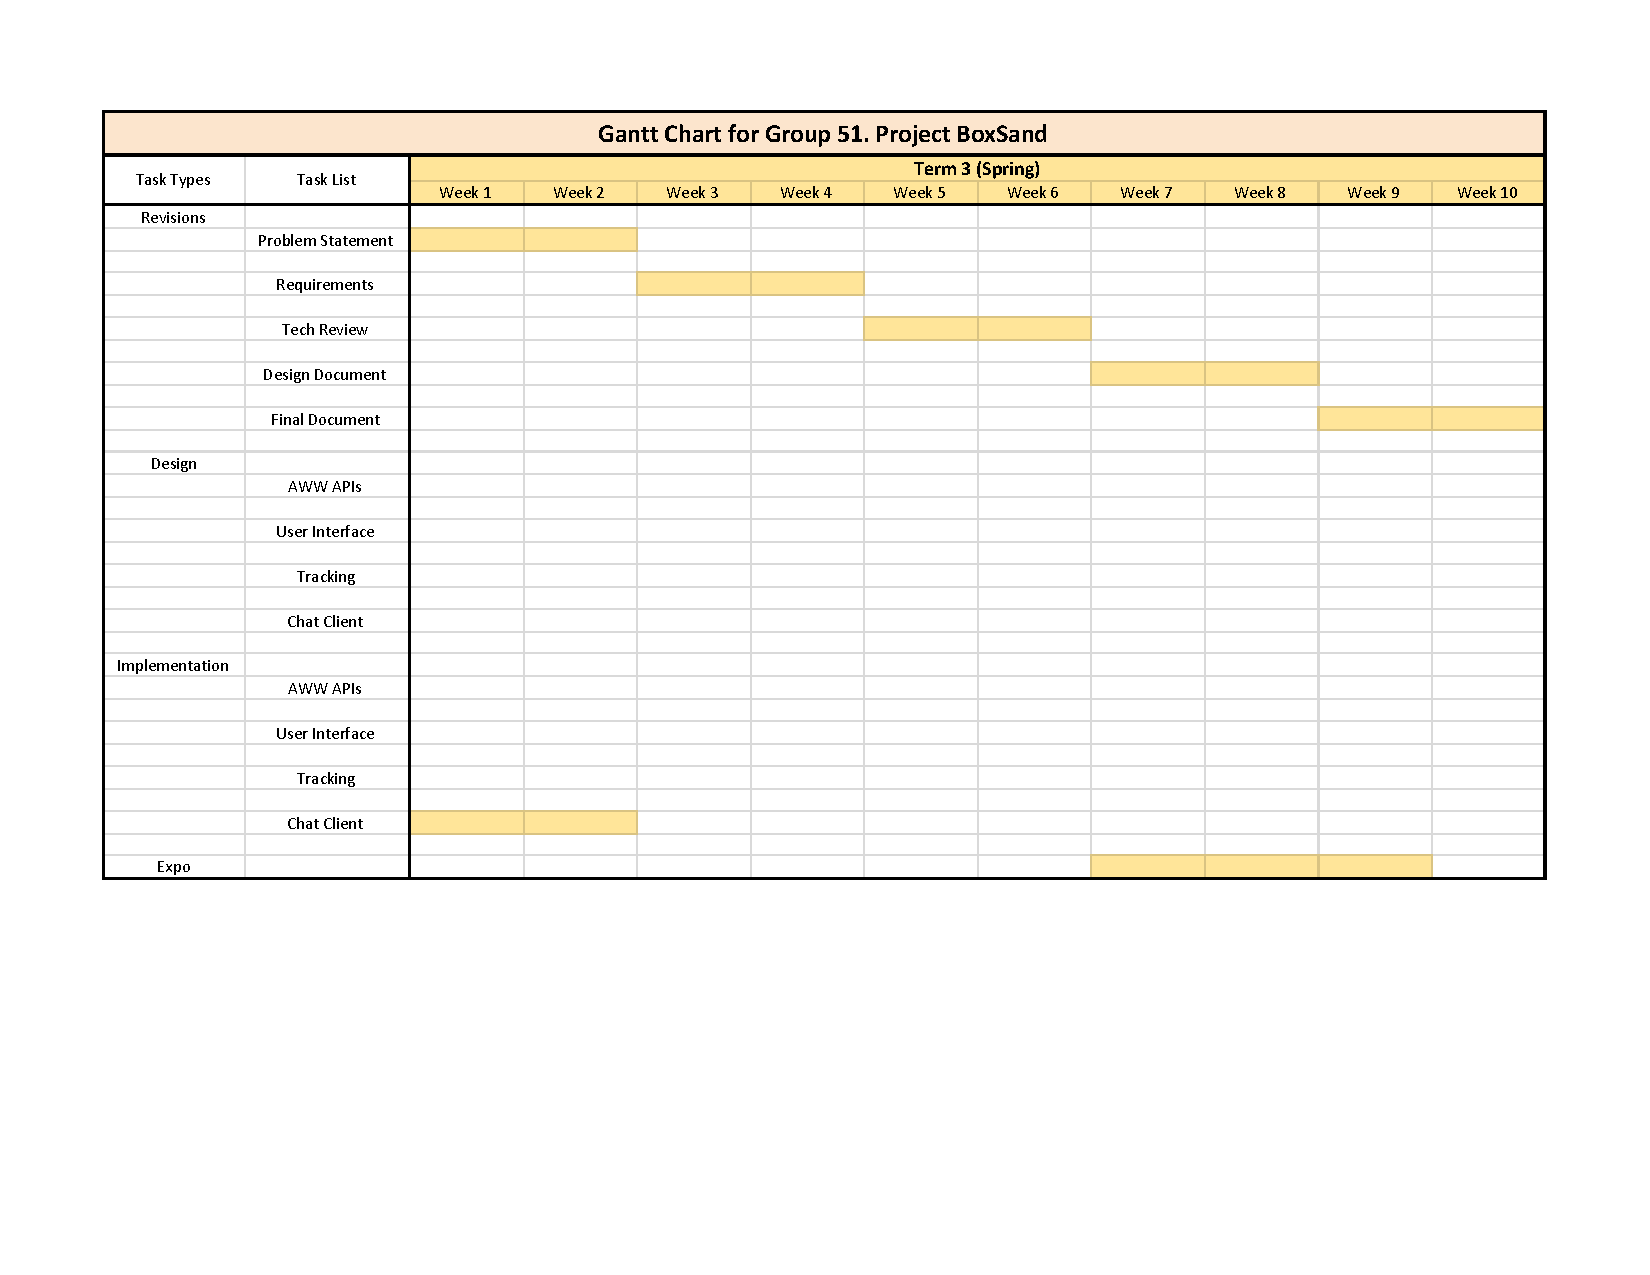
\includegraphics[width=7in]{Simplified Gantt Chart - Term 3.pdf}
		\end{center}
	\end{figure}

\end{document}
